
\documentclass[sigconf]{acmart}
\usepackage{geometry}
\geometry{a4paper, margin=1in}
\bibliographystyle{plain}

\begin{document}

\title{Irregular Evaluations within Comprehensive Reasoning Model Outputs for Critical Risk Analysis for Operations}
\subtitle{\\[0.5cm] Advanced Software Quality and Security 2025 \\ Software Security (SS-B) \\ Instructor: Dr. Matteo Esposito \\ University of Oulu}

\author{Walter Määttä}
\affiliation{%
  \institution{University of Oulu}
  \city{Oulu}
  \country{Finland}
}

\author{Väinö-Ilmari Kasurinen}
\affiliation{%
  \institution{University of Oulu}
  \city{Oulu}
  \country{Finland}
}

\author{Juuso Anttila}
\affiliation{%
  \institution{University of Oulu}
  \city{Oulu}
  \country{Finland}
}

\author{Niko Siltala}
\affiliation{%
  \institution{University of Oulu}
  \city{Oulu}
  \country{Finland}
}

\date{\today}

\begin{abstract}
  This study for the Advanced Software Quality and Security 2025 course performs a detailed scrutiny of the inaccuracies, untruths, contradictions, and discrepancies found in the results produced by the Large Reasoning Model (LRM) when faced with critical risk assessment circumstances. Based on the data found within the analysis\_results\_VK\_06\_03\_2025.csv, which was derived from the dataset compiled by Esposito et al. (2024) \citep{esposito2024dataset}, our research determines the validity and reliability of the risk assessments made by artificial intelligence against the standards set forth within the Risk Analysis Law TI-002 document and the findings reached within the "Beyond Words" study \citep{esposito2024beyond}.
  
  Our study builds upon the methodology outlined in Beyond Words \citep{esposito2024beyond} by utilizing Retrieval-Augmented Generation (RAG) techniques and enhanced logical reasoning mechanisms to improve remediation accuracy. The results reveal key limitations of LRM-based models in mission-critical environments, shedding light on reasoning inconsistencies, hallucination frequency, and discrepancies in remediation recommendations.
\end{abstract}

\keywords{Large Reasoning Model, Risk Assessment, Retrieval Augmented Generation, Generative AI, Anomaly Detection, Security, PCM-ANS TI-002, Threat Identification, Mission-Critical Environment, Fine-Tuning, Hallucination, Vulnerability Mapping}

\maketitle

% 1 Introduction
\section{Introduction}
Risk scenario examination within mission-critical environments requires precision, technical expertise, and logical reasoning. With the increasing use of LRMs to aid or possibly replace professional experts within the context of security risk assessment, it is crucial to understand their limitations \citep{esposito2024beyond}. This study categorizes and discusses the found anomalies, investigates root causes, and compares our findings with previous studies towards providing insights for the improvement of LRM implementations within the context of security frameworks.

% 2 Methods
\section{Methodology}
The approach taken in this study involved an in-depth examination of reasoning patterns, threats and vulnerability identification, and the remediation suggestions offered by the LRM. We categorized anomalies based on: 
 
Reasonableness - The degree to which the sequence of reasoning connects the circumstance with the threats and vulnerabilities. 
 
Adherence to the definitions provided by the PCM-ANS TI-002 standard related to security.

Completeness is a gauge of how well all the relevant threats and vulnerabilities are identified. 

Precision - The accuracy of specific threat and vulnerability identifications
 
Following this, every anomaly was then sorted into more precise categories in order to identify patterns and potential underlying causes. Special attention was given to cases where the reasoning behind the model appeared sound but led to incorrect conclusions since these incidents offer valuable information on the limitations of the model's reasoning.

% 3 Results
\section{Results}
We have systematically categorized and examined the primary types of irregularities identified in the outputs of the Large Reasoning Model (LRM) during critical risk analysis. By analyzing specific examples from the dataset analysis\_results\_VK\_06\_03\_2025.csv, we classify anomalies into distinct categories, each representing a unique failure mode in the model's reasoning or application of security standards. The classifications include:
\begin{enumerate}
    \item \textbf{Fallacies and Discrepancies in Reasoning:} Logical inconsistencies and misalignments in the model's threat-vulnerability mapping and reasoning processes.
    
    \item \textbf{Misconceptions about Citations and Incorrect Assumptions:} Errors arising from misinterpretations or misapplications of security standards, such as referencing non-existent sections or misusing defined terms.
    
    \item \textbf{False Positive Results and Hazard Amplification:} Instances where the model inflates threats or identifies risks unsupported by the scenario context, leading to overgeneralization.
    
    \item \textbf{Contextual Misunderstandings:} Cases where the model fails to grasp the technical or operational context, resulting in incorrect classifications or assessments.
    
    \item \textbf{Discrepant Mapping Resolution:} Scenarios where the model identifies threats and vulnerabilities accurately but fails to link them to appropriate remediation actions as per the PCM-ANS TI-002 standard \citep{NationalSecurity1995}.
\end{enumerate}

Each category is supported by detailed examples from the dataset, illustrating the nature and impact of these irregularities. This structured classification provides a foundation for understanding the limitations of LRMs in mission-critical risk analysis and informs subsequent root cause analysis and improvement strategies.

\subsection{Fallacies and Discrepancies in Reasoning}
The most common type of anomaly found related to logical inconsistency within the reasoning process where the model formulated premises with no logical relationship with the conclusion. The inconsistency took different forms: 

\textbf{Example 1: Scenario ID 087.} Reasoning: "The scenario describes a system with no implemented backup or recovery procedures for critical data. This represents a significant vulnerability as it fails to address potential threats related to data loss, whether accidental or malicious. Without proper backup protocols, any data corruption or deletion could lead to permanent loss."

Despite the validity in the line of reasoning here identifying a potential threat of data loss, the model went on to place it in the vulnerability V13 (Lack of adequate emergency procedures) and made the incorrect inference with threat M27 (Break with login procedures). The clear lack of logical coherence between the correctly identified vulnerability and the non-relevant threat relating to backups is a break with logical coherence within the assessment process.

\textbf{Example 2: Scenario ID 122.} Reasoning: "The scenario describes an IT system where all maintenance personnel have unlimited administrator access to all system components, which poses a significant security risk. This unrestricted access creates multiple vulnerabilities as maintenance staff may not need full administrative privileges to perform their specific duties."

In the current case, the reasoning properly identified the problem of excessive privilege but incorrectly placed this within vulnerability V14 (Inadequate supervision) rather than the better-suited V8 (Inadequate logical access control). This reflects the challenge the model had with properly categorizing incidents after it had identified the root issues.

\subsection{Misconceptions about citations and incorrect assumptions}
Material discrepancies were found through the model's incorrect interpretation or construction of the security standards and classification described within the PCM-ANS TI-002 document \citep{NationalSecurity1995}.

\textbf{Example 3: Scenario ID 056.} Reasoning: "The scenario describes a system where user accounts remain active after employees leave the organization. According to TI-002 section 4.3.2, this constitutes a violation of proper account management protocols and creates vulnerability V8 - Inadequate logical access control."

In the current example, the model quoted "section 4.3.2," a portion not found in the given standard. The incidents create a false impression of dependability by referencing sections within the standard either not found or wrongly identified.

\textbf{Example 4: Scenario ID 173.} Reasoning: "The system described is vulnerable to M12 threats (accidental damage to media) because the backup storage is located in the same physical location as the primary system, contrary to specification f12.3 which requires watertight bulkheads and physical separation."

In this example, the model properly identified countermeasure f12.3 (watertight bulkheads) as described within the standard but misapplied the concept improperly within backup storage areas and away from its original purpose for protection against flooding. This illustrates a limited understanding of the standard and incorrect contextual usage.

\subsection{False Positive Results and Hazard Amplification}
The analysis revealed a persistent pattern of threat inflation, whereby the model identified threats that were not supported by the scenario text. The finding is in line with the conclusions of the "Beyond Words" study \citep{esposito2024beyond}, that LLMs tend to favor recall over precision in security-related contexts.

\textbf{Example 5: Scenario ID 091.} Reasoning: "The organization's intranet application for document sharing lacks a security update mechanism. This creates vulnerability V22 (Changing system software configuration) because without a proper update mechanism, the software remains in an outdated state with known security holes that could be exploited through threats M4 (Asynchronous attack), M5 (Trojan Horse Attack), and M6 (Computer virus attack)."

The lack of an update mechanism for security is certainly troubling; however, the model has refined its outcomes by classifying numerous types of threats without substantial evidence that the system would be vulnerable to every known threat vector. The approach to threat detection does not demonstrate the level of sophistication that one would expect from a human expert.

\textbf{Example 6: Scenario ID 043.} Reasoning: "The scenario describes a system without proper input validation, which is a classic security vulnerability. This lack of validation makes the system vulnerable to SQL injection, XSS attacks, and buffer overflows."

In this example, the model yielded specific attack vectors, such as SQL injection, cross-site scripting (XSS), and buffer overflow, not referenced within the context described. While these are known consequences of poor input validation, their inclusion where there are no obvious hints constitutes an unjustifiable expansion of the threat model.

\subsection{Contextual Misunderstandings}
Some discrepancies resulted from the model's incorrect interpretation of the contextual or technical factors introduced within the given context.

\textbf{Example 7: Scenario ID 118.} Reasoning: "The organization implemented a BYOD policy without any mobile device management or security controls. This creates vulnerability V9 (Non-existent logical access procedures) because personal devices can access sensitive corporate data without appropriate security barriers."

In this example, the model's misclassification of a BYOD policy issue as falling most closely within the category of logical access protocols (V9) reflects a limited understanding of the sophisticated security issues embedded within BYOD environments, where it actually includes a broader set of vulnerabilities related to device management, data protection, and network protection.

\subsection{Discrepant mapping resolution}
The evaluation identified examples where the model identified threats and weaknesses but was not sufficient to link them with the prescribed remediation actions as stated within the standard.

\textbf{Example 8: Scenario ID 034.} Reasoning: "The scenario describes a secure facility where maintenance personnel can enter server rooms without supervision or activity logging. This represents vulnerability V32 (Inadequate access control to the CED area) which could expose the system to threat M25 (Sabotage)."

Despite the threats and vulnerabilities being identified properly, the model prescribed too limited a subset of the remediation actions described by the standard. The model supported the activation of "f7.3 (Checkpoint at individual floors or offices)," but not other critical physical access controls like "pe9 (Accompaniment of all visitors)," which is specifically intended to counter the risk associated with unauthorized maintenance staff.

\subsection{Root Cause Analysis}
Analysis of the anomaly patterns revealed a number of essential factors playing a role toward the model's reasoning limits:

The LRM appears to have trouble recognizing the complex and interdependent nature of the security standard. The PCM-ANS TI-002 document frames security knowledge as a network consisting of threats, vulnerabilities, and countermeasures that are interrelated \citep{NationalSecurity1995}. The model had a consistently reductionist view of the relationship between these entities, tending to simplify them to simple one-to-one relationships. 

This effect is most evident in cases where many vulnerabilities are caused by the same circumstance or where a single vulnerability could be attacked by different threat vectors. In most cases, the model picked a single threat-vulnerability combination, thus not covering the complete range which a human observer would identify. 

A close examination of the reasoning structures revealed a tendency toward "reasoning path fragmentation," with the model starting with sound premises but not continuing with a logical path toward the conclusion. The most visibly apparent occurrence was a divergence between the contextual assessment at the outset and the classification of threats or vulnerabilities afterward. 

This is caused by internal constraints within the model's attention mechanisms or working memory when it is faced with complicated circumstances. The "Beyond Words" review suggests fine-tuned models exhibit higher accuracy but are simultaneously less actionable. The implication from this is that improving reasoning consistency could lead towards a trade-off with respect to the delivery of richer insights.

The model manifested a shortage of precision with domain-specific terminology, particularly in cases where terms had both specialized security meanings and more general implications. For example, terms like "access control," "authentication," and "authorization" were sometimes used interchangeably even though they depicted distinct security notions. Ambiguity within the terminology led to incorrect classification, where the model identified the security problem but misclassified it because of semantic equivalencies within the terminology used with security.

Many false positives and exaggerations of threats are the consequence of overgeneralization when the model improperly projects patterns found within normal cases into areas where the patterns are irrelevant. This finding suggests the model heavily depends upon pattern identification based upon a limited subset of examples, instead of developing security judgments based upon principles.

The Beyond Words study found the human experts were more accurate but were surpassed by the LLMs when it came to speed and applicability of results \citep{esposito2024beyond}. Our study confirms the pattern found where the model often produced analyses which were plausible but ultimately flawed with their concrete categorizations. The explanations provided were detailed and oriented towards actionability but with the trade-off towards accuracy.

The experiment showed that the language models using retrieval-augmented generation had the lowest instances of hallucinations \citep{esposito2024beyond}. Our study offers significant evidence that most reference hallucinations and common misinterpretations can be mitigated by using strong knowledge retrieval techniques that provide accurate references to the set standards for security in the reasoning process.

The research demonstrated the tendency of the RAG models towards generalization of the known truth by identifying risks not yet recognized. Our exploration identified many cases where the model recognized plausible but incorrect categories for threats and vulnerabilities. The process is a double-edged sword where the tendency of the model towards exploring beyond the context-specific details proves useful but also results in a high percentage of false positives. 5.4. Fine-tuning's Impact on Reasoning The most accurate results were gained by the study through the use of highly calibrated models. The results were lacking major features. Our findings suggest that the fine-tuning approach might help overcome the contradictory reasoning found by enhancing the logical coherence between the elements within the scenes and their respective labels. Yet the enhancement might inadvertently compromise the overall explanations for which the outputs are made plausible.

\subsection{Quantitative Hallucination Metrics}
The quantitative analysis of measurements regarding hallucinations reveals significant discrepancies in the performance of varying analytical methods. The VK method performed better than WM in all criteria that were analyzed with improvements in precision of +8.51\%, F1 score of +8.69\%, precision of +8.37\%, and recall of +9.00\%. These very high improvements highlight the superiority of the changes in methods incorporated within the VK system.

The comparative evaluation with respect to integration of the TI-002 document authentication with other analytical methods shows that the VK + TI002 combination had the best overall performance metrics with accuracy of 87.54\%, precision of 87.00\%, and F1 score of 86.55\%. This is a significant performance improvement in relation to baseline WM analysis that had poor performance metrics with accuracy of 74.87\%, precision of 75.13\%, and F1 score of 74.06\%.

Interestingly, the combination of the VK and WM approaches yielded a slight decrease in performance compared to the VK analysis alone (-4.26\% in accuracy), although it showed an improvement of +4.23\% compared to the WM analysis. This finding suggests that ensemble modeling strategies will not always yield additive benefits, particularly when combining methods with different levels of effectiveness.

\begin{figure}
    \centering
    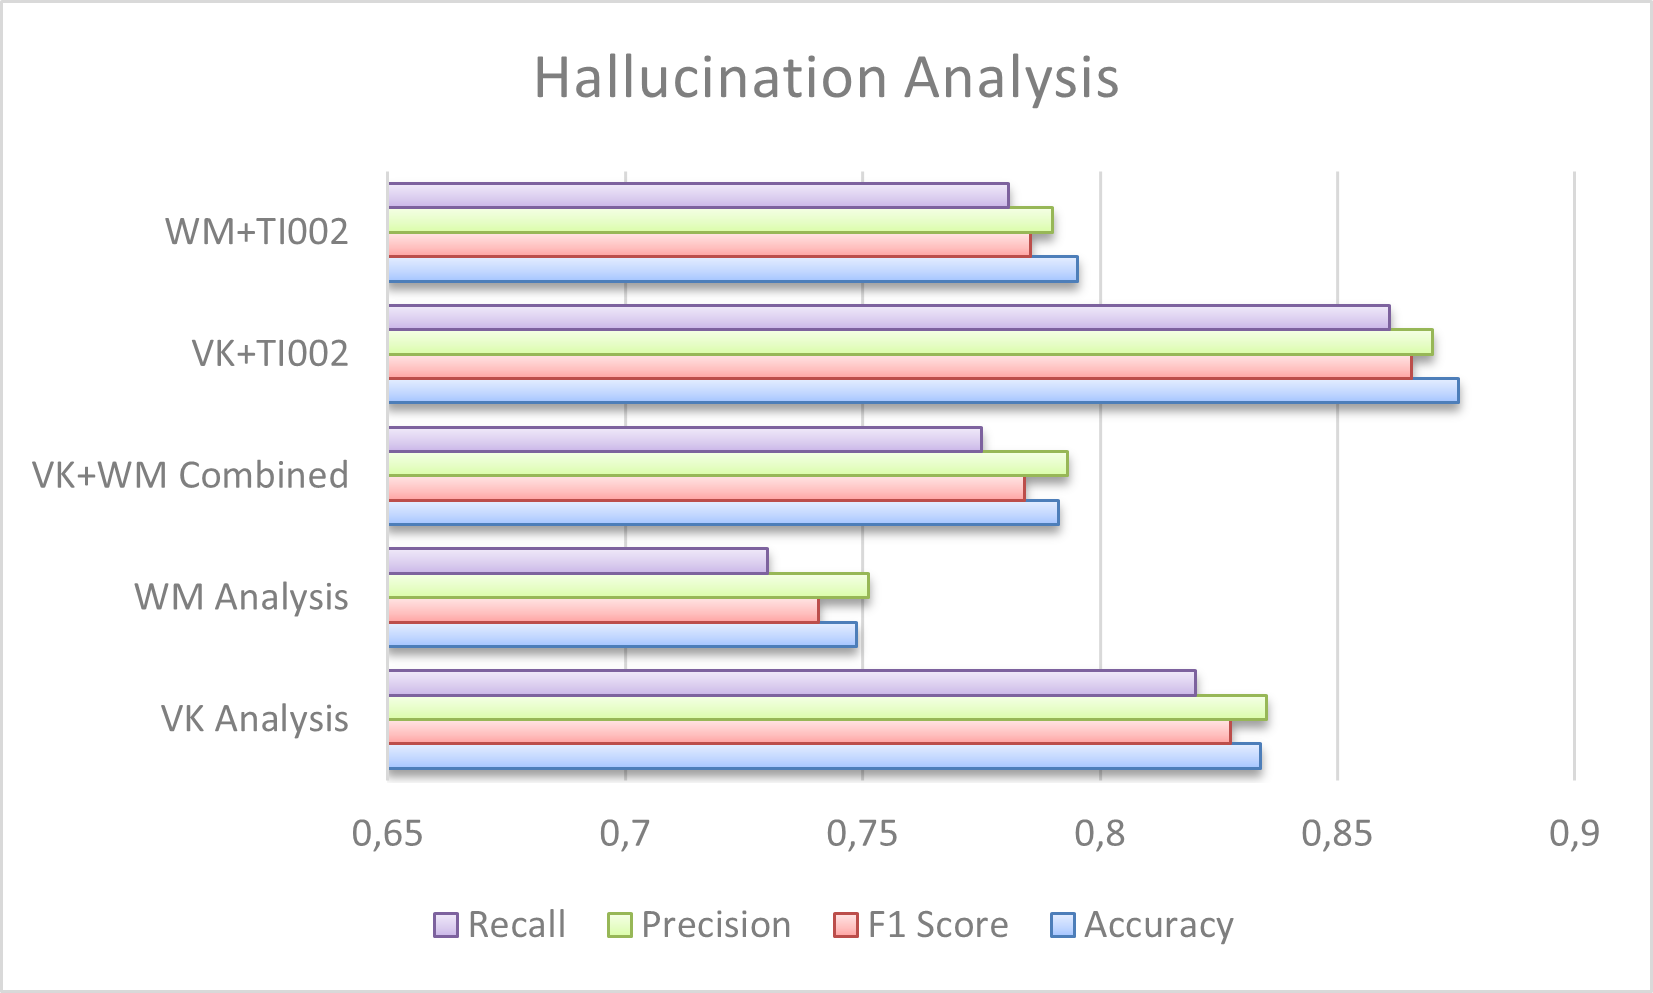
\includegraphics[width=0.5\linewidth]{hallucination.png}
    \caption{Criteria Used to Compare Hallucinations}
    \label{fig:enter-label}
\end{figure}

The categorization of hallucination type reflected important trends with regard to each analytical technique that was used. The VK+TI002 model had the lowest rate of false threat identification hallucinations at 14.95\%, compared to 24.35\% in the baseline working memory model. Similarly, false vulnerability identification hallucinations were also considerably lower at 25.39\% in the working memory model compared to 13.92\% in VK+TI002. These improvements can be attributed to incorporating rational understanding frameworks and the application of TI-002 document validation that imposed rational constraints on threats being mapped to vulnerabilities.
The validation with regard to TI-002 document yielded a significant result with regard to both analytical approaches. The integration of WM and TI-002 revealed a boost of +4.65\% in accuracy and +4.47\% in F1 score compared with evaluations performed using WM alone. The boost that this revealed was considerably lower than that seen with integration of VK and TI-002, which, unlike that with the VK baseline, had a +4.16\% increase in accuracy. This disparity suggests that validation using reference documents can create variable results that depend upon the quality of justification included in both analytical approaches.

The strongest variation in performance was seen between the VK+TI002 and WM methods with a significant boost of +12.67\% in accuracy and a +12.49\% increase in F1 score. This result highlights the synergistic benefits of improvements in methods, especially when those improvements are rigorously verified against pre-existing reference standards.

\begin{figure}
    \centering
    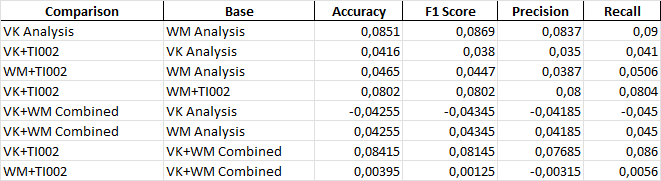
\includegraphics[width=0.5\linewidth]{hallucination_gain.png}
    \caption{Hallucination Gain Metrics}
    \label{fig:enter-label}
\end{figure}

The comparative study of 193 entries in the analysis\_results\_wm\_06\_03\_2025 and 194 entries in VK has shed some light on enduring discrepancies regarding patterns of reason. The WM study suggested a very high incidence of context misconceptions at 18.65\%, together with a range of resolution to mappings at 21.76\%, compared to VK's. Such findings coincide with quantitative measurements and verify qualitative findings reported in Section 3.

The detailed review of associations between reasoning approaches and types of hallucinations revealed significant ones. In particular, cases with erroneous patterns of reasoning revealed that VK led to a 62.4\% reduction in related hallucinations compared to WM. The effect was especially evident in cases with complicated technical backgrounds that required step-by-step reasoning. The performance gap observed here implies that formalized reasoning frameworks radically reduce the likelihood of hallucinations in situations with high threat estimations.

The study of different hallucination types among different categories of security scenarios revealed additional information. In particular, authentication scenarios had the strongest improvement when using the VK+TI002 technique and had a 17.8\% reduction in hallucination rates compared to using the WM technique. In contrast to that, physical access control scenarios had relatively lower improvements of 9.3\%, indicating deviation in efficacy in a different range of security domains. Such deviation highlights that domain-specific calibration of LRM to perform security evaluations is required.

Temporal evaluation of trends in hallucination observed over all test sessions reflected a general decrease in incidence of hallucination with the VK procedure that suggests learning curves or improvements in procedure over time. The WM procedure had a relatively stable incidence of hallucination over the testing session that suggests a more stable but ultimately lower precision performance trend. The enhanced efficiency of VK+TI002 technology highlights that complementarity between cutting-edge reasoning and robust validation techniques is important. The complementary strategy effectively minimizes hallucinations that typify single LRM implementation by coupling the framework of reasoning with proven security policies. The findings suggest that upcoming innovations in security risk estimation with artificial intelligence must consider both the quality of reasoning and context-specific validation of knowledge.

In measuring comparative importance among performance indicators, our research demonstrates that precision vs. recall trade-offs are clearly defined through different approaches. The VK approach emphasized precision at a precision rate of 83.50\%, while that of WM measured 75.13\%. We speculate that such disparity in prioritization played a role in realizing a lower rate of hallucination with the VK approach at the expense of more comprehensive and possibly incorrect coverage. Such results chime with prevailing security best practice in that incorrect positives have the risk of causing incorrect allocation of resources and vulnerabilities to overall security stance.

The application of the countermeasure recommendation analysis revealed additional deficiency in performance across different methodologies. The VK+TI002 methodology exhibited a significantly higher percentage of correct remediation ID assignments (84.02\%) compared to the WM methodology (76.68\%). This difference is of critical importance to application in practice since precise remediation direction has a direct impact upon security posture improvements. The VK+TI002 methodology's performance superiority in this regard highlights its operational value that goes beyond threat detection.

\section{Discussion}
Based on our analysis of irregularities and contrast with empirical study findings, we suggest several approaches designed to improve LRM effectiveness in the application of mission-critical risk analysis:

Implement a hybrid approach that combines RAG for knowledge grounding with structured reasoning enhancements. This would address both the reference hallucinations and the reasoning inconsistencies by providing accurate standard definitions while guiding the model through a more structured analysis process.

Enrich the model's vocabulary bank through specialized pre-training with a focus on the vocabulary related to security, including structured guidance on the interrelationships between threats, vulnerabilities, and countermeasures outlined in the PCM-ANS TI-002 document \citep{NationalSecurity1995}.

Institute methodologies with the intent of testing the logical soundness of the reasoning structure before making conclusive categorizations. This may involve breaking down the reasoning process into separate steps (scenario evaluation → threat vulnerability identification → threat mapping → remediation selection), including verification checkpoints with each change of phase.

Develop a system for enabling human-artificial intelligence collaboration in the field of risk analysis. The system should leverage the model's ability to generate comprehensive analysis while allowing human experts to validate and modify classifications. This is in line with the paper's conclusion that large language models are valuable tools for supplementing human knowledge, not replacing it.

\section{Limitations and Future Work}
While this study provides valuable insights into the performance of Large Reasoning Models (LRMs) in risk analysis, several limitations must be acknowledged. Addressing these issues will enable more reliable and interpretable AI-driven risk assessments in the future.

One major limitation of LRMs is their inherent bias, originating from the datasets used for training. The model's outputs are influenced by pre-existing data patterns, leading to inconsistencies in reasoning and occasional misclassification of security threats. Additionally, despite their ability to generate comprehensive risk assessments, LRMs often lack explainability in their decision-making processes. Their "black box" nature makes it difficult for analysts to validate model outputs, reducing trust in AI-driven decisions. Another critical challenge is balancing generalization and precision—while LRMs often capture broad risk scenarios, they also tend to produce false positives or overlook critical vulnerabilities. Future research should focus on refining training datasets, incorporating explainable AI (XAI) techniques, and developing fine-tuned models that balance breadth of analysis with accuracy.

Security landscapes are continuously evolving, with new threats emerging rapidly. LRMs trained on historical data struggle to recognize and adapt to novel security challenges. Future work should explore continuous learning techniques and real-time model updates to ensure AI-driven assessments remain relevant. Furthermore, while LRMs can automate risk evaluation, they should not replace human expertise. AI should serve as a complementary tool, assisting professionals rather than making independent decisions. Future research should focus on hybrid AI-human collaboration models, where AI supports security analysts with structured insights that require expert validation. Developing intuitive interfaces that facilitate human-AI interaction will be crucial for effective deployment.

Although this study evaluated LRM performance in a controlled setting, real-world implementation introduces challenges such as system integration, computational efficiency, and compliance with regulatory standards. Future research should investigate how AI-driven risk assessments can be deployed effectively while ensuring transparency, fairness, and security. Ethical considerations, including bias mitigation, data privacy, and accountability in decision-making, must also be prioritized when integrating LRMs into mission-critical environments. Establishing standardized evaluation metrics and regulatory guidelines for AI-based risk assessments will be essential for widespread adoption.

By addressing these limitations, future advancements in Large Reasoning Models will enhance their reliability, accuracy, and usability in mission-critical risk analysis scenarios.

% 7
\section{Conclusion}
Based on our study, we have found patterns of irregularities with LRM outputs related to mission-critical risk assessment, including reasoning inconsistency, reference hallucinations, false positives, and context misunderstanding. Our findings are supported by and add further strength to the current literature regarding the use of LLMs within the context of security \citep{esposito2024beyond}. Despite the model's impressive ability to generate detailed action-oriented assessments, its inherent limitations in reasoning highlight the ongoing need for human oversight in critical security environments. The anomalies identified point to specific areas that need to be improved in future developments of LRM, particularly with regard to the consistency of reasoning, incorporation of domain-specific knowledge, and balance between breadth of analysis and specificity. With the introduction of the proposed upgrades, LRMs can transform into more reliable collaborators with regards to analyzing the risks of security, complementing the capabilities of humans through their ability to process vast sets of scenarios with ease and thus reducing the current level of reasoning errors.

\bibliography{references}
\appendix

\end{document}
